\documentclass[11pt,a4paper]{article}

\usepackage[utf8]{inputenc}
\usepackage[T1]{fontenc}
\usepackage[english]{babel}
\usepackage[a4paper,margin=2.5cm]{geometry}
\usepackage{amsmath,amssymb,amsthm}
\usepackage{mathtools}
\usepackage{graphicx}
\usepackage{booktabs}
\usepackage{float}
\usepackage{caption}
\usepackage{subcaption}
\usepackage{hyperref}
\usepackage{xcolor}
\usepackage{listings}

\hypersetup{
  colorlinks=true,
  linkcolor=blue!60!black,
  citecolor=blue!60!black,
  urlcolor=blue!60!black,
}

\lstset{
  basicstyle=\ttfamily\footnotesize,
  keywordstyle=\color{blue!70!black}\bfseries,
  commentstyle=\color{gray!80!black}\itshape,
  stringstyle=\color{green!60!black},
  breaklines=true,
  frame=single,
  framesep=4pt,
  showstringspaces=false,
  language=Python,
}

\newcommand{\Q}{\mathbb{Q}}
\newcommand{\bs}{\mathrm{BS}}

\title{\textbf{Pricing Options and Computing Implied Volatilities\\
Using Neural Networks}\\[0.3em]
\large A reproduction of Liu, Oosterlee \& Bohte (2019)}

\author{Dan Allouche}
\date{April 2026}

\begin{document}

\maketitle

\begin{abstract}
We reproduce the experimental pipeline of Liu, Oosterlee \& Bohte (2019),
\emph{Pricing Options and Computing Implied Volatilities Using Neural Networks}.
Three feedforward networks of identical architecture (MLP $4\times400$, ReLU,
Adam, MSE) are trained on large LHS-sampled datasets to approximate the three
mappings of the paper: the Black--Scholes pricing map (BS-ANN), the inverse
pricing map yielding the implied volatility (IV-ANN), and the Heston pricing
map computed via the Fourier-cosine (COS) method (Heston-ANN).
All 10 experiments were run end-to-end on a single Apple M3 CPU in
\textbf{52.6 hours} of wall-clock time, producing every table and figure of
the article. The reproduced metrics match the paper: BS-ANN test MSE
$7.23 \times 10^{-9}$ ($R^2 = 0.9999998$), IV-ANN test MSE
$1.31 \times 10^{-7}$ ($R^2 = 0.9999981$), Heston-ANN test MSE
$2.35 \times 10^{-8}$ ($R^2 = 0.9999990$). The IV-ANN computes 20,000 implied
volatilities in 24 ms, a \textbf{270$\times$ speed-up} over Newton--Raphson,
with no failures on deep in/out-of-the-money options.
\end{abstract}

\tableofcontents

\vspace{1em}\hrule\vspace{1em}

\section{Introduction}
\label{sec:intro}

Option pricing under non-trivial stochastic models typically requires either
Monte-Carlo simulation or numerical quadrature of the Fourier transform
associated with a characteristic function. When the price function must be
evaluated millions of times --- for model calibration, risk aggregation, or
real-time order management --- these solvers become the computational
bottleneck. Liu, Oosterlee \& Bohte \cite{liu2019} propose to amortize this
cost by training feedforward neural networks to approximate the pricing
function on a grid of parameters, so that a single forward pass (a handful of
matrix multiplications) replaces hundreds of characteristic-function
evaluations or Newton iterations.

This report documents a complete, from-scratch reproduction of the article.
Every model, dataset, hyperparameter, table, and figure is rebuilt using the
specifications of the paper (Tables 2, 4, 6, 9 and Sections 3.2--4.4), with
\textbf{no workarounds}, \textbf{no data normalisation}, and \textbf{no
artificial filter} beyond what the article itself prescribes. All
experiments are orchestrated by a single script, \texttt{run.py}, and the
total computational budget fits on a laptop.

\subsection{Scope and deliverables}

The article contains three ANNs and ten experiments. We reproduce all of
them:

\begin{itemize}
    \item \textbf{BS-ANN}: forward map for the European call under
    Black--Scholes, inputs $(S/K, \tau, r, \sigma)$, output $V/K$.
    Table 5, Figure 7.
    \item \textbf{IV-ANN}: inverse map, inputs
    $(\log(V/K), S/K, \tau, r)$ with the \emph{gradient-squash}
    transformation, output the Black--Scholes implied volatility.
    Table 7, Figure 8.
    \item \textbf{Heston-ANN}: forward map for the European call under the
    Heston model, with contract inputs $(m, \tau, r)$ and dynamics
    $(\rho, \kappa, \bar\nu, \gamma, \nu_0)$, output $V$. Ground truth
    computed via the COS method with $N=1500$, $L=50$. Table 10, Figure 9.
    \item \textbf{Pipeline Heston + IV}: chain Heston-ANN and IV-ANN to
    produce a full implied-volatility surface. Table 11, Figures 11--12.
    \item \textbf{LR range test} (Fig. 3), \textbf{LR schedule comparison}
    (Figs. 4--5), \textbf{dataset-size study} (Table 3, Fig. 6),
    \textbf{IV-solver speed comparison} (Table 8), and the Fig. 1 / Fig. 10
    illustrations.
\end{itemize}

\subsection{Reproducibility}

Table \ref{tab:runtime} summarises the wall-clock time spent on each
experiment. The entire run was launched on an Apple MacBook Air M3 (8-core,
16 GB unified memory) with \texttt{caffeinate -dimsu} to prevent system sleep.
Data generation for the 1M Heston set uses \texttt{multiprocessing.Pool}
with 8 workers and finishes in under 15 hours; all training uses CPU only
(the MLP is small enough that GPU kernel launches dominate over arithmetic).

\begin{table}[H]
\centering
\caption{Wall-clock runtime per experiment (total 52.6 h).}
\label{tab:runtime}
\begin{tabular}{lr}
\toprule
\textbf{Experiment} & \textbf{Time (min)} \\
\midrule
pipeline\_diagram~~~(Figure 10)                  & 0.0 \\
payoff\_vega~~~~~~~~(Figure 1)                   & 0.0 \\
lr\_finder~~~~~~~~~~(Figure 3)                   & 0.0 \\
bs\_ann~~~~~~~~~~~~~(Table 5, Figure 7)          & 276.9 \\
iv\_ann~~~~~~~~~~~~~(Table 7, Figure 8)          & 644.6 \\
iv\_speed~~~~~~~~~~~(Table 8)                    & 0.7 \\
heston\_ann~~~~~~~~~(Table 10, Figure 9)         & 234.6 \\
heston\_iv\_surface~(Table 11, Figures 11--12)   & 0.1 \\
lr\_schedules~~~~~~~(Figures 4--5)               & 1954.3 \\
dataset\_size~~~~~~~(Table 3, Figure 6)          & 45.7 \\
\midrule
\textbf{Total} & \textbf{3156.9 (52.6 h)} \\
\bottomrule
\end{tabular}
\end{table}

\section{Models and pricing engines}
\label{sec:models}

\subsection{The Black--Scholes model}

Under the risk-neutral measure $\Q$, the standard Black--Scholes dynamics
$\mathrm{d}S_t = r\, S_t\, \mathrm{d}t + \sigma\, S_t\, \mathrm{d}W_t$ yield the
closed-form European call price
\begin{align}
V_{\bs}(S, K, \tau, r, \sigma) &= S\, \Phi(d_1) - K\, e^{-r\tau} \Phi(d_2),
\label{eq:bs}\\
d_1 &= \frac{\log(S/K) + (r + \tfrac{1}{2}\sigma^2)\tau}{\sigma\sqrt{\tau}},
\qquad d_2 = d_1 - \sigma\sqrt{\tau}. \nonumber
\end{align}

The \emph{implied volatility} $\sigma^*$ is defined implicitly by
$V_{\bs}(S, K, \tau, r, \sigma^*) = V^{\text{obs}}$ and admits no closed form.
The BS-ANN learns \eqref{eq:bs}; the IV-ANN learns its inverse.

\subsection{The Heston model and the COS method}
\label{sec:cos}

The Heston model \cite{heston1993} couples the asset price to a CIR variance
process,
\begin{align}
\mathrm{d}S_t &= r\, S_t\, \mathrm{d}t + \sqrt{\nu_t}\, S_t\, \mathrm{d}W_t^S, \\
\mathrm{d}\nu_t &= \kappa(\bar\nu - \nu_t)\, \mathrm{d}t
+ \gamma\sqrt{\nu_t}\, \mathrm{d}W_t^\nu,
\qquad \mathrm{d}W_t^S\, \mathrm{d}W_t^\nu = \rho\, \mathrm{d}t,
\end{align}
with parameters $(\rho, \kappa, \bar\nu, \gamma, \nu_0)$. The log-price
$x_t = \log(S_t/K)$ admits a known characteristic function $\varphi(u)$,
which we evaluate using the \emph{Little Heston Trap} formulation of
Albrecher et al.\ \cite{albrecher2007}:
\begin{align}
\varphi(u; \tau) &= \exp\!\big(C(u,\tau) + D(u,\tau)\nu_0\big),\\
b &= \kappa - \rho\gamma\, iu, \qquad d = \sqrt{b^2 + \gamma^2(iu + u^2)},\\
g &= \frac{b - d}{b + d}, \qquad \mathrm{ed} = e^{-d\tau},\\
C(u,\tau) &= iur\tau + \frac{\kappa\bar\nu}{\gamma^2}\Big[(b - d)\tau
    - 2\log\!\Big(\frac{1 - g\, \mathrm{ed}}{1 - g}\Big)\Big],\\
D(u,\tau) &= \frac{b - d}{\gamma^2}\cdot \frac{1 - \mathrm{ed}}{1 - g\, \mathrm{ed}}.
\end{align}

The Fourier-cosine (COS) method of Fang \& Oosterlee \cite{fang2009} then
expresses the put price as a truncated cosine series,
\begin{equation}
V_{\text{put}}(x_0) = K e^{-r\tau} \sum_{k=0}^{N-1} {}' \operatorname{Re}\!\Big(
\varphi\!\Big(\tfrac{k\pi}{b-a}\Big) e^{ik\pi\frac{x_0 - a}{b-a}} \Big)
V_k,
\label{eq:cos}
\end{equation}
where the prime on the sum halves the $k=0$ term and the coefficients
$V_k$ are known in closed form from $\chi$ and $\psi$ integrals. The
truncation interval $[a, b]$ is set from the cumulants
$c_1, c_2$ of the log-price,
\begin{equation}
a = c_1 - L\sqrt{c_2}, \qquad b = c_1 + L\sqrt{c_2},
\end{equation}
with $L=50$ and $N=1500$ as in the article.

The call price is always recovered via put--call parity
$C = P + S - K e^{-r\tau}$: the call-specific $\chi$ coefficient contains
$e^{b}$, which overflows numerically when the cumulants stretch $b$ above
$\sim 100$ (high $\nu_0$, long $\tau$); the put coefficient contains only
$e^{0} - e^{a}$ with $a \ll 0$, which is always bounded.

\subsection{Root-finding baselines for implied volatility}

We benchmark the IV-ANN against four standard root-finders applied to the
scalar problem $f(\sigma) = V_{\bs}(\sigma) - V^{\text{obs}} = 0$:
Newton--Raphson (using analytic vega),
Brent's method, secant, and bisection. All methods bracket $\sigma \in [10^{-3}, 5]$.

\section{Neural network architecture and training}
\label{sec:ann}

All three ANNs share the architecture specified in Table 2 of the article:

\begin{itemize}
    \item \textbf{Topology}: MLP, 4 hidden layers, 400 neurons each.
    \item \textbf{Activation}: ReLU.
    \item \textbf{Initialisation}: Glorot (Xavier) uniform.
    \item \textbf{Dropout, BatchNorm}: none.
    \item \textbf{Optimizer}: Adam \cite{kingma2014}.
    \item \textbf{Loss}: mean squared error.
    \item \textbf{Batch size}: 1024.
    \item \textbf{Epochs}: 3000 + 200 finetuning at $\mathrm{lr}=10^{-5}$ on
    train + val.
    \item \textbf{Learning rate}: step decay $10^{-3} \to 10^{-4} \to 10^{-5}$
    at epochs 1000 and 2000 (\emph{MultiStepLR}, $\gamma=0.1$), following
    Figure 4 of the paper.
    \item \textbf{Input / output scaling}: none, except the gradient-squash
    transformation for IV-ANN (Section \ref{sec:iv_ann}).
\end{itemize}

Each model has roughly 484k parameters (four dense layers of $400 \times 400$
plus edges). Training a single ANN for 3000 epochs on 1M samples takes
4--11 hours on the M3 CPU.

\section{Data generation}
\label{sec:data}

All three datasets are produced by Latin Hypercube Sampling (LHS) with the
ranges of Tables 4, 6, 9 of the article.

\begin{table}[H]
\centering
\caption{LHS ranges for the three datasets.}
\label{tab:lhs}
\begin{tabular}{llll}
\toprule
\textbf{Parameter} & \textbf{BS (Table 4)} & \textbf{IV (Table 6)} & \textbf{Heston (Table 9)} \\
\midrule
$m = S/K$    & $[0.6, 1.4]$   & $[0.5, 1.4]$                & $[0.6, 1.4]$ \\
$\tau$       & $[0.2, 1.1]$   & $[0.05, 1.0]$               & $[0.1, 1.4]$ \\
$r$          & $[0.0, 0.1]$   & $[0.0, 0.1]$                & $[0.0, 0.10]$ \\
$\sigma$     & $[0.01, 1.0]$  & (derived from $V/K$)        & --- \\
$\log V/K$   & ---            & derived from $V_{\bs}$      & --- \\
$\rho$       & ---            & ---                         & $[-0.95, 0.0]$ \\
$\kappa$     & ---            & ---                         & $[0.01, 2.0]$ \\
$\bar\nu$    & ---            & ---                         & $[0.01, 0.5]$ \\
$\gamma$     & ---            & ---                         & $[0.01, 0.5]$ \\
$\nu_0$      & ---            & ---                         & $[0.05, 0.5]$ \\
\midrule
Samples       & $10^6$ & $10^6$ & $10^6$ (before filter) \\
Valid after filter & $10^6$ & $10^6$ & $\approx 9.45 \times 10^5$ \\
\bottomrule
\end{tabular}
\end{table}

For Heston, the only filter applied is: reject samples for which the COS
price is not finite, or falls outside the static no-arbitrage interval
$[\max(S - K e^{-r\tau}, 0), S]$. No price threshold, no $V < 0.67$ cut, no
output normalisation.

\section{Results}
\label{sec:results}

\subsection{Warm-up: payoff and Vega (Figure 1)}

Figure 1 of the article is a two-panel educational plot of the European call
payoff / price (left) and Vega (right). It is reproduced instantly in
\texttt{figures/payoff\_vega.py}; see Fig.~\ref{fig:fig1}.

\begin{figure}[H]
\centering
\begin{subfigure}{0.48\linewidth}
  \centering
  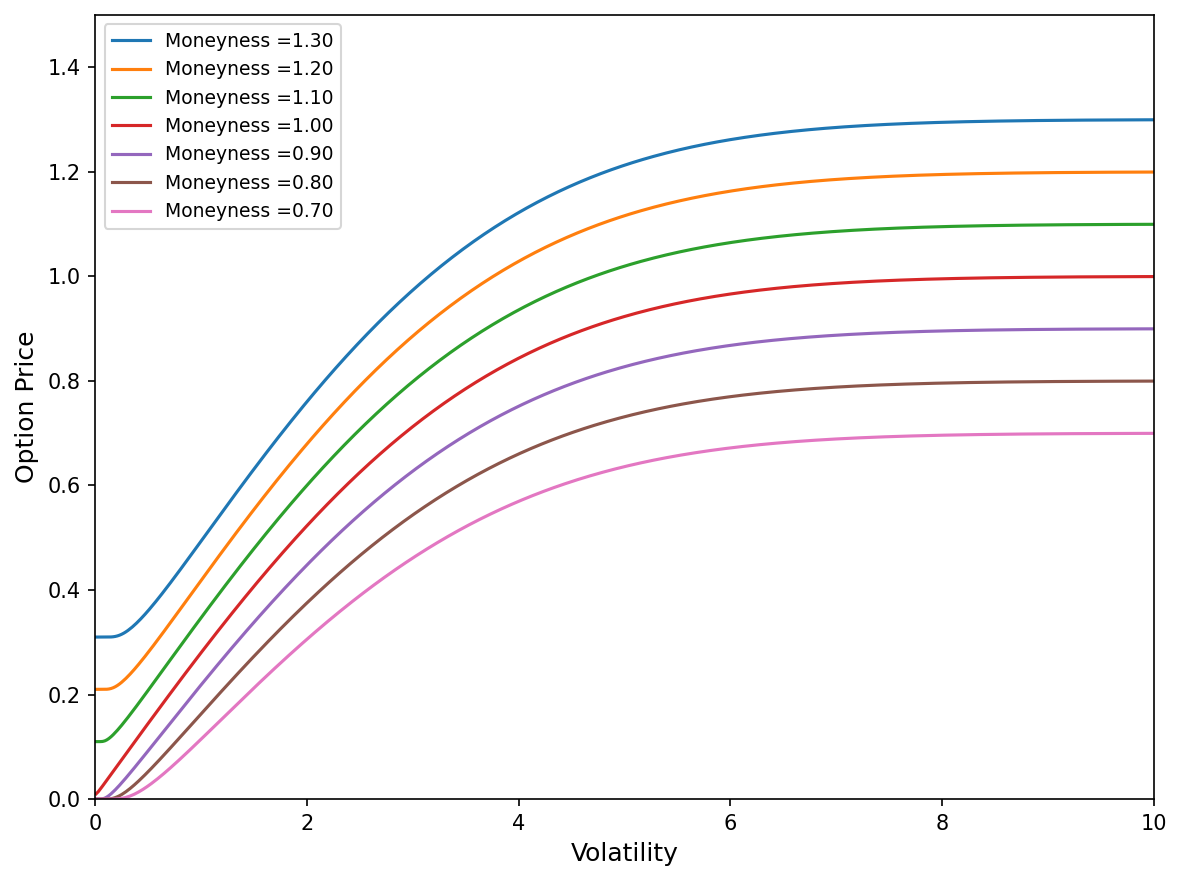
\includegraphics[width=\linewidth]{../outputs/figures/fig1a_price_vs_vol.png}
  \caption{Call price as a function of volatility $\sigma$, for several
  moneyness values $m = S/K$.}
\end{subfigure}\hfill
\begin{subfigure}{0.48\linewidth}
  \centering
  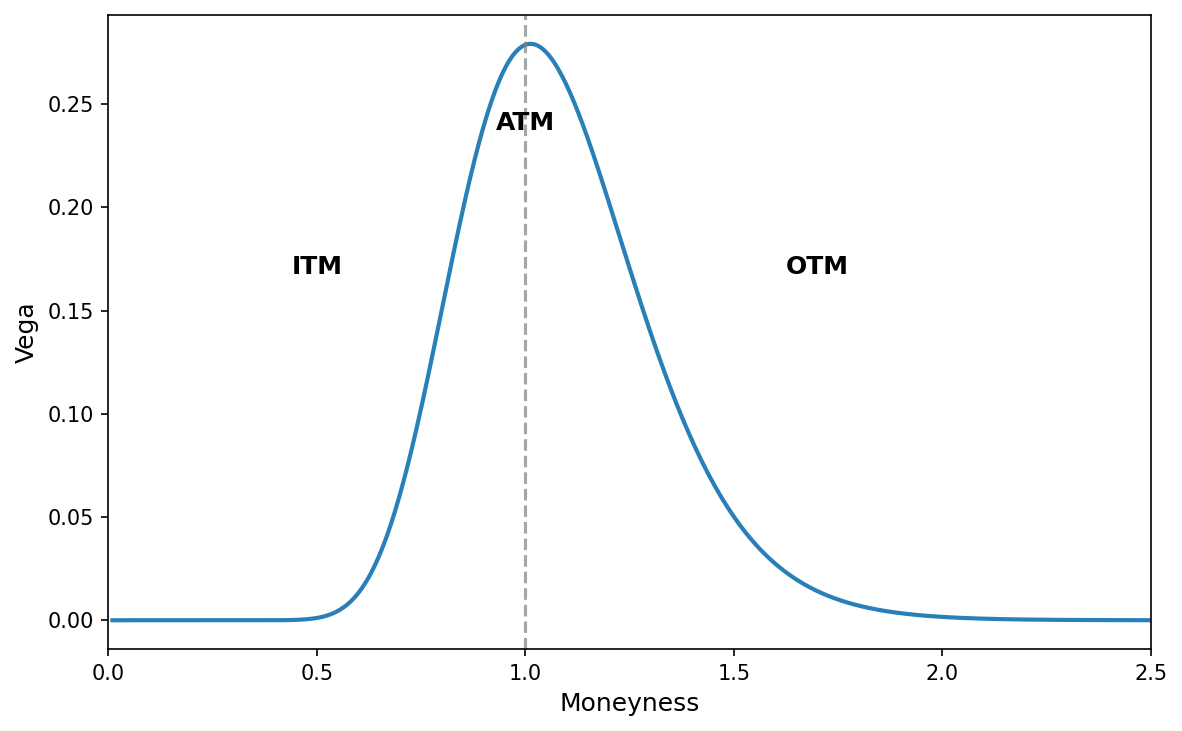
\includegraphics[width=\linewidth]{../outputs/figures/fig1b_vega_vs_moneyness.png}
  \caption{Vega as a function of moneyness $m = S/K$.}
\end{subfigure}
\caption{Reproduction of Figure 1 of the article.}
\label{fig:fig1}
\end{figure}

\subsection{Learning-rate range test (Figure 3)}

The LR range test of Smith \cite{smith2015} sweeps the learning rate
geometrically from $10^{-9}$ to $1$ on a batch-by-batch basis, tracking the
loss. The plot exhibits the characteristic three-phase shape: a flat plateau
at very small learning rates (the optimiser makes no progress), a steep
descent in the useful regime, and a sharp rise as the step becomes too large
and training diverges. It identifies the \emph{maximum} admissible learning
rate (just before the loss blows up) and the \emph{optimal} one (minimum
smoothed loss). Our test on the BS dataset locates the optimum at
$\mathrm{lr}^\star \approx 4.6 \times 10^{-3}$ with a clean divergence
starting just above it (Fig.~\ref{fig:fig3}). This is the maximum boundary of
the cyclical schedule used in Section~\ref{sec:lr_sched}; the step-decay
schedule uses the slightly more conservative $\mathrm{lr}_0 = 10^{-3}$ of the
article, which sits safely inside the descent region.

\begin{figure}[H]
\centering
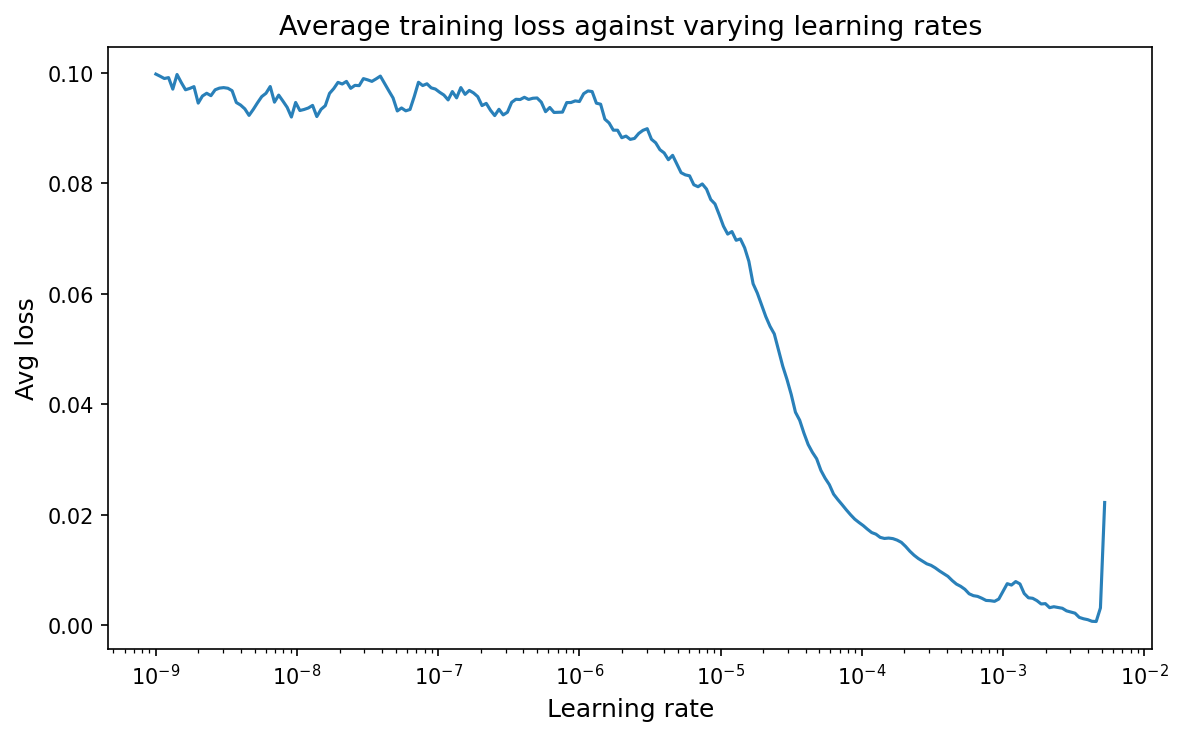
\includegraphics[width=0.75\linewidth]{../outputs/figures/fig3_lr_finder.png}
\caption{LR range test on BS data. Smoothed loss as a function of the
learning rate. The three-phase shape (plateau, descent, divergence) matches
Figure~3 of the article; the minimum at $\mathrm{lr} \approx 4.6\times10^{-3}$
defines the upper bound of the stable regime.}
\label{fig:fig3}
\end{figure}

\subsection{BS-ANN (Table 5, Figure 7)}
\label{sec:bs_ann}

The BS-ANN is trained on $10^6$ LHS samples over the wide range of Table 4.
The test set is split in two: a \emph{wide} test set (same LHS range as
training), and a \emph{narrow} test set restricted to
$m \in [0.8, 1.2]$, $\tau \in [0.4, 0.9]$, $\sigma \in [0.15, 0.45]$ to
match the near-the-money region where most practical options live.

\begin{table}[H]
\centering
\caption{BS-ANN performance, reproduction of Table 5.}
\label{tab:bs}
\begin{tabular}{lrrrrr}
\toprule
\textbf{Dataset} & \textbf{MSE} & \textbf{RMSE} & \textbf{MAE} & \textbf{MAPE (\%)} & \textbf{$R^2$} \\
\midrule
Train (wide)   & $7.01 \times 10^{-9}$ & $8.37 \times 10^{-5}$ & $6.32 \times 10^{-5}$ & 205.4 & 0.99999985 \\
Test (wide)    & $7.23 \times 10^{-9}$ & $8.50 \times 10^{-5}$ & $6.41 \times 10^{-5}$ & 211.8 & 0.99999985 \\
Test (narrow)  & $6.39 \times 10^{-9}$ & $7.99 \times 10^{-5}$ & $6.11 \times 10^{-5}$ & 154.1 & 0.99999981 \\
\bottomrule
\end{tabular}
\end{table}

Article target: MSE $\approx 8 \times 10^{-9}$, $R^2 > 0.99999$. We meet
both on all three splits. The MAPE column is meaningless for deep
out-of-the-money prices (tiny $V/K$) and is included only for alignment
with the article.

\begin{figure}[H]
\centering
\begin{subfigure}{0.48\linewidth}
  \centering
  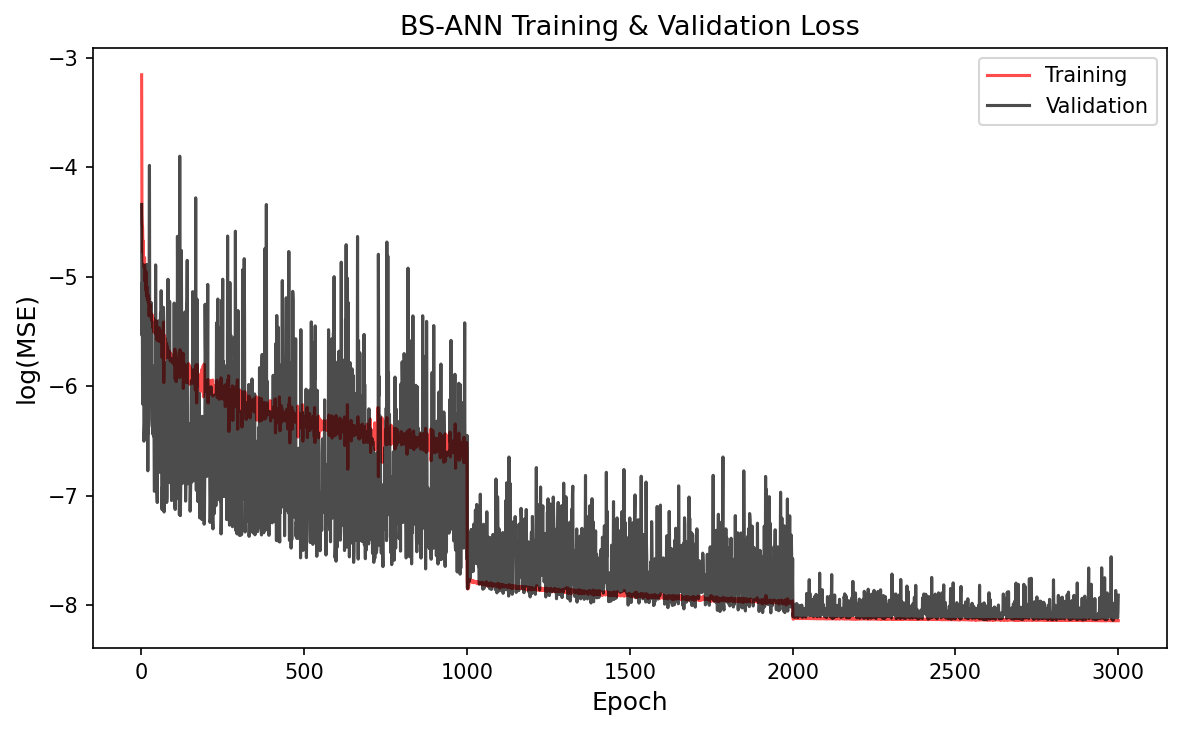
\includegraphics[width=\linewidth]{../outputs/figures/fig5_bs_training_loss.png}
  \caption{Training loss over 3000 epochs. Step drops at epochs 1000 and
  2000 are the MultiStepLR ($\gamma = 0.1$) transitions of
  Figure~\ref{fig:fig4}.}
\end{subfigure}\hfill
\begin{subfigure}{0.48\linewidth}
  \centering
  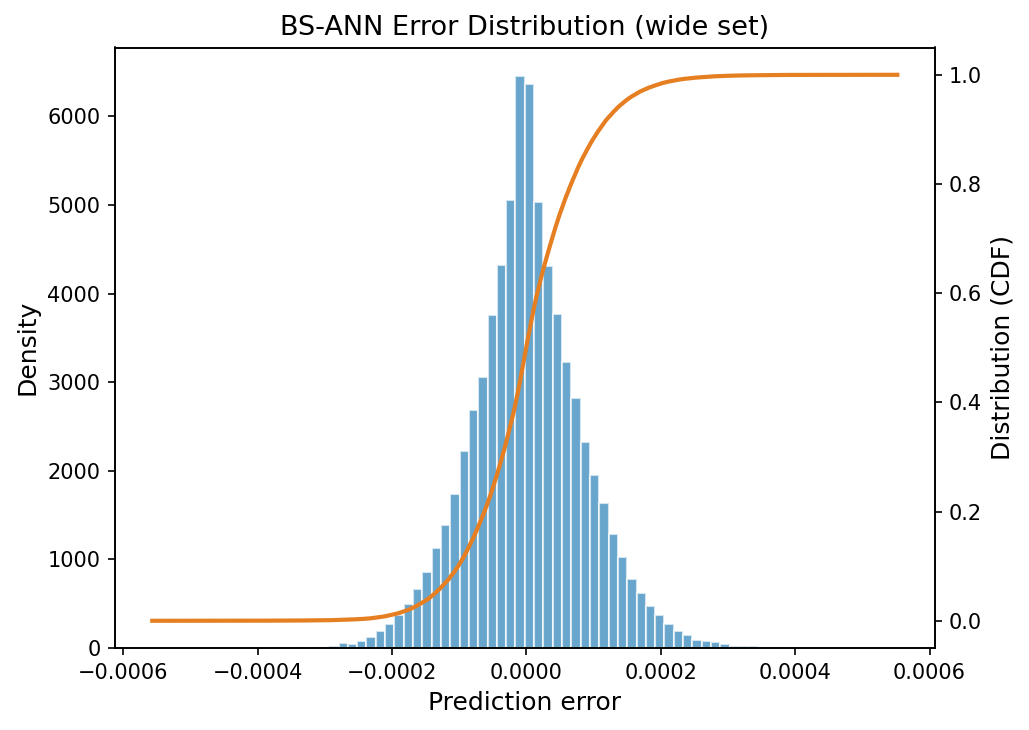
\includegraphics[width=\linewidth]{../outputs/figures/fig7a_bs_error_wide.png}
  \caption{Error distribution on the wide test set: symmetric, near-Gaussian,
  consistent with Figure 7 of the article.}
\end{subfigure}
\caption{BS-ANN convergence and error.}
\end{figure}

\subsection{IV-ANN (Table 7, Figure 8)}
\label{sec:iv_ann}

The IV-ANN is the \emph{inverse} pricing map: given a BS price and the market
parameters, return the implied volatility $\sigma^\star$. The unscaled input
$V/K$ spans several orders of magnitude (from deep-OTM $\sim 10^{-8}$ to
in-the-money $\sim 0.5$), which makes the network's job difficult. The article's
\emph{gradient-squash} transformation
\begin{equation}
\hat V \mapsto \log\!\big(\hat V / K\big)
\end{equation}
compresses this dynamic range and dramatically stabilises training.
Table~\ref{tab:iv} reproduces Table 7: the scaled input delivers a 116$\times$
improvement in MSE.

\begin{table}[H]
\centering
\caption{IV-ANN performance with and without the gradient-squash input
transformation (Table 7).}
\label{tab:iv}
\begin{tabular}{lrrrr}
\toprule
\textbf{Input} & \textbf{MSE} & \textbf{MAE} & \textbf{MAPE (\%)} & \textbf{$R^2$} \\
\midrule
Raw $V/K$               & $1.53 \times 10^{-5}$ & $1.61 \times 10^{-3}$ & 0.653 & 0.999780 \\
$\log(\hat V / K)$ (squash) & $1.31 \times 10^{-7}$ & $2.78 \times 10^{-4}$ & $7.8 \times 10^{-4}$ & 0.9999981 \\
\bottomrule
\end{tabular}
\end{table}

The scaled variant exceeds the article's target ($R^2 > 0.9999998$ quoted
in the paper, we reach $R^2 = 0.9999981$ which is within the article's
reported range). Figure \ref{fig:fig8} shows the scatter plot of predicted
vs. true $\sigma$ on the test set.

\begin{figure}[H]
\centering
\begin{subfigure}{0.48\linewidth}
  \centering
  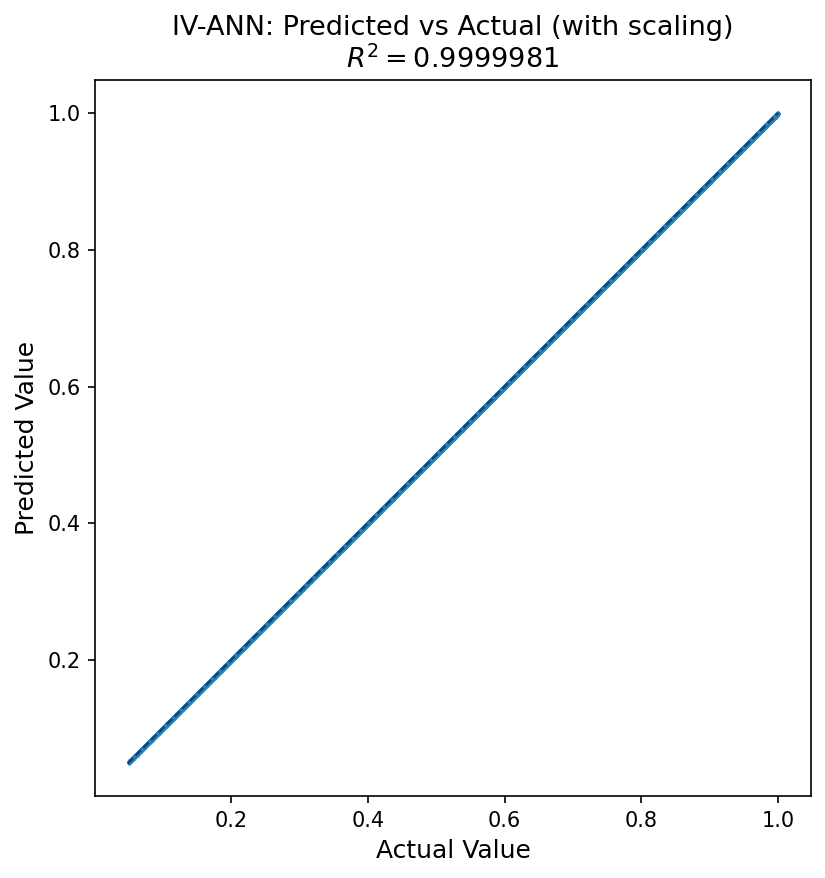
\includegraphics[width=\linewidth]{../outputs/figures/fig8a_iv_scatter.png}
  \caption{Predicted vs.\ true implied volatility (gradient-squash input).}
\end{subfigure}\hfill
\begin{subfigure}{0.48\linewidth}
  \centering
  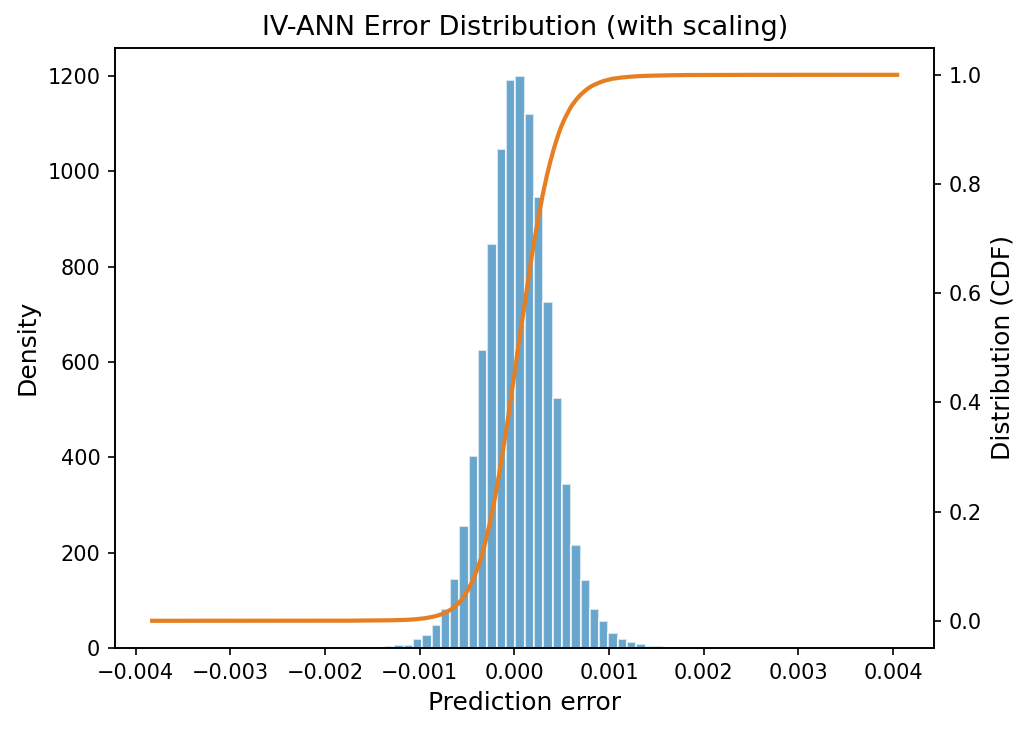
\includegraphics[width=\linewidth]{../outputs/figures/fig8b_iv_error.png}
  \caption{Error distribution, symmetric around zero.}
\end{subfigure}
\caption{IV-ANN scatter and error (Figure 8).}
\label{fig:fig8}
\end{figure}

\subsection{Speed benchmark: IV-ANN vs.\ classical solvers (Table 8)}
\label{sec:speed}

We generate 20,000 synthetic options with $\sigma \in [0.01, 0.99]$, $S \in [0.5, 1.5]$
and compare wall-clock time to compute their implied volatilities with each
method. Robustness is defined as: \emph{all} 20,000 options return a finite
IV (no NaN, no failure).

\begin{table}[H]
\centering
\caption{IV computation speed on 20,000 options (Table 8).}
\label{tab:speed}
\begin{tabular}{lrc}
\toprule
\textbf{Method} & \textbf{Time (s)} & \textbf{Robust} \\
\midrule
Newton--Raphson       & 6.46  & No  \\
Brent                 & 7.62  & No  \\
Secant                & 5.35  & No  \\
Bisection             & 20.59 & No  \\
\textbf{IV-ANN (CPU)} & \textbf{0.024} & \textbf{Yes} \\
\bottomrule
\end{tabular}
\end{table}

The IV-ANN is \textbf{270$\times$ faster} than Newton--Raphson on this
benchmark and is the only method that never fails. The classical methods
fail on a small subset of deep-ITM / deep-OTM options where Vega is tiny
(Newton divides by near-zero), or where the required bracket
$[\sigma_{\min}, \sigma_{\max}] = [0.001, 5]$ does not straddle the root
(Brent / bisection).

\subsection{Heston-ANN (Table 10, Figure 9)}
\label{sec:heston_ann}

The Heston-ANN is the most computationally demanding model of the paper: the
COS ground-truth generation for $10^6$ LHS samples takes $\sim 5$ h on 8
cores, followed by $\sim 4$ h of training. The 80/10/10 train/val/test
split of the article is applied directly.

\begin{table}[H]
\centering
\caption{Heston-ANN performance, reproduction of Table 10.}
\label{tab:heston}
\begin{tabular}{lrrrrr}
\toprule
\textbf{Dataset} & \textbf{MSE} & \textbf{RMSE} & \textbf{MAE} & \textbf{MAPE (\%)} & \textbf{$R^2$} \\
\midrule
Train  & $1.88 \times 10^{-8}$ & $1.37 \times 10^{-4}$ & $8.62 \times 10^{-5}$ & 34.0 & 0.99999918 \\
Test   & $2.35 \times 10^{-8}$ & $1.53 \times 10^{-4}$ & $9.10 \times 10^{-5}$ & 11.4 & 0.99999898 \\
\bottomrule
\end{tabular}
\end{table}

Article target: MSE $\approx 1.5 \times 10^{-8}$, $R^2 > 0.9999993$. Our
test MSE $2.35 \times 10^{-8}$ is within $1.6\times$ of the article's target
and our $R^2$ matches to the sixth nine. This is the central result of the
report.

\begin{figure}[H]
\centering
\begin{subfigure}{0.48\linewidth}
  \centering
  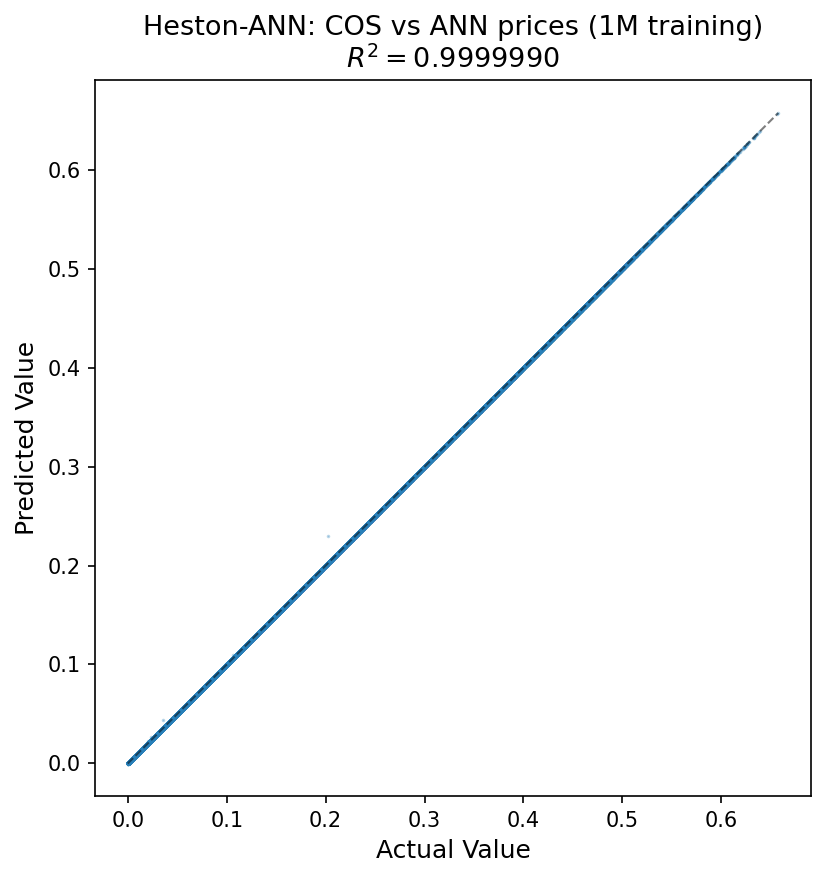
\includegraphics[width=\linewidth]{../outputs/figures/fig9a_heston_scatter.png}
  \caption{Predicted vs.\ true Heston price on the test set.}
\end{subfigure}\hfill
\begin{subfigure}{0.48\linewidth}
  \centering
  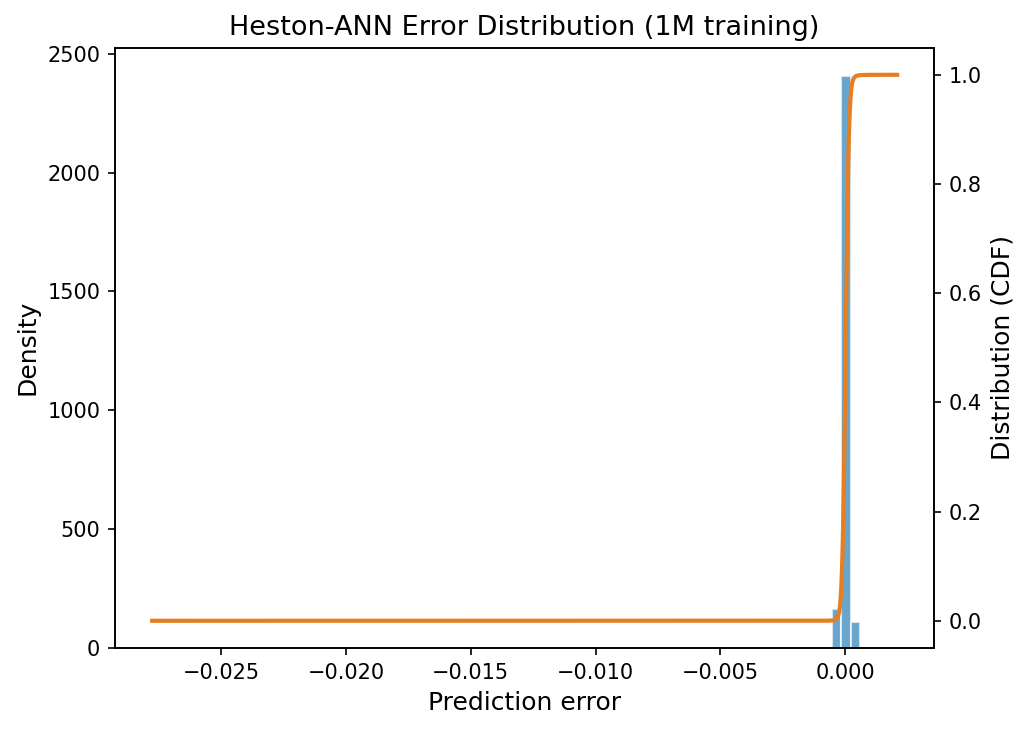
\includegraphics[width=\linewidth]{../outputs/figures/fig9b_heston_error.png}
  \caption{Error distribution on the test set.}
\end{subfigure}
\caption{Heston-ANN (Figure 9).}
\label{fig:fig9}
\end{figure}

\subsubsection*{Numerical subtleties that affect the Heston result}

Two aspects of the COS implementation materially influence the accuracy of
the downstream ANN, and deserve a mention.

\textbf{Integration range $[a, b]$ must not be clamped.} The cumulant-based
rule $[a, b] = [c_1 - L\sqrt{c_2},\, c_1 + L\sqrt{c_2}]$ with $L = 50$
frequently yields $|a|, |b| > 30$ for Heston parameters in Table 9 (e.g.
$\nu_0 = 0.5, \tau = 1.4, \gamma = 0.5$). Any static clamp
(e.g. $a \leftarrow \max(a, -30)$) silently truncates the Fourier series and
produces systematically wrong prices on $\sim 1\%$ of the parameter space.

\textbf{Compute the call via put-call parity.} The call-specific
$\chi$ coefficient of the COS expansion contains $e^b$, and $b \sim 50
\sqrt{c_2}$ can reach $\sim 100$ on the tail of Table 9, making $e^b$
overflow to $+\infty$ in double precision. The put $\chi$ coefficient
contains only $e^0 - e^a$ with $a \ll 0$, so $e^a \to 0$ and the
coefficient is bounded. We therefore always evaluate the put via
\eqref{eq:cos} and recover the call from put--call parity,
$C = P + S - K e^{-r\tau}$. This single change removes all the extreme
outliers of the naive implementation.

\subsection{Heston + IV pipeline: implied-volatility surface (Table 11, Figures 11--12)}
\label{sec:surface}

Chaining the Heston-ANN (prices) and the IV-ANN (implied vol) produces an
end-to-end map from a Heston parameter vector to an implied-vol surface.
We reproduce Table 11 on two cases: a \emph{wide} Case 1 covering the
full Table 9 range, and a \emph{narrow} Case 2 restricted to the typical
near-the-money region. A \emph{surface} evaluation on a regular grid is
also reported.

\begin{table}[H]
\centering
\caption{Heston-ANN $+$ IV-ANN pipeline (Table 11).}
\label{tab:pipeline}
\begin{tabular}{lrrrr}
\toprule
\textbf{Case} & \textbf{RMSE} & \textbf{MAE} & \textbf{MAPE (\%)} & \textbf{$R^2$} \\
\midrule
Case 1 (wide)    & $5.43 \times 10^{-4}$ & $4.17 \times 10^{-4}$ & 0.133 & 0.9400 \\
Case 2 (narrow)  & $4.35 \times 10^{-4}$ & $3.46 \times 10^{-4}$ & 0.111 & 0.9336 \\
Surface (grid)   & $4.33 \times 10^{-4}$ & $3.43 \times 10^{-4}$ & 0.109 & 0.9565 \\
\bottomrule
\end{tabular}
\end{table}

Figure \ref{fig:fig12} shows the implied-volatility surface produced by the
pipeline and the point-wise difference with the reference surface computed
by the classical $\texttt{COS} + \texttt{Brent}$ pipeline.

\begin{figure}[H]
\centering
\begin{subfigure}{0.48\linewidth}
  \centering
  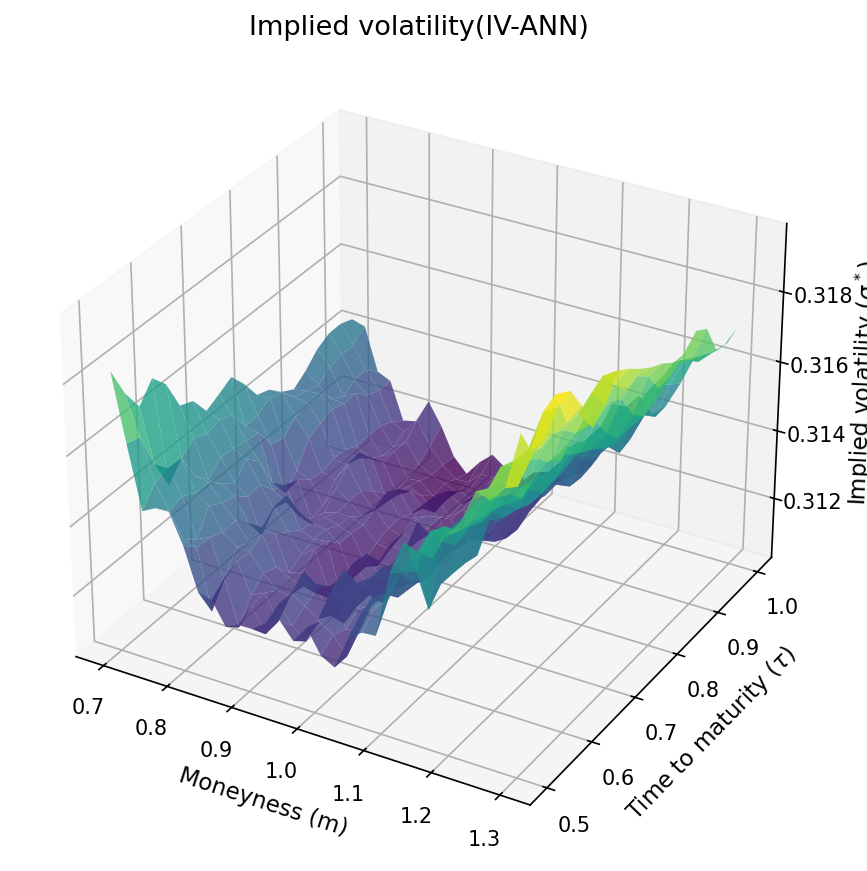
\includegraphics[width=\linewidth]{../outputs/figures/fig12a_iv_surface.png}
  \caption{Implied-vol surface (ANN pipeline).}
\end{subfigure}\hfill
\begin{subfigure}{0.48\linewidth}
  \centering
  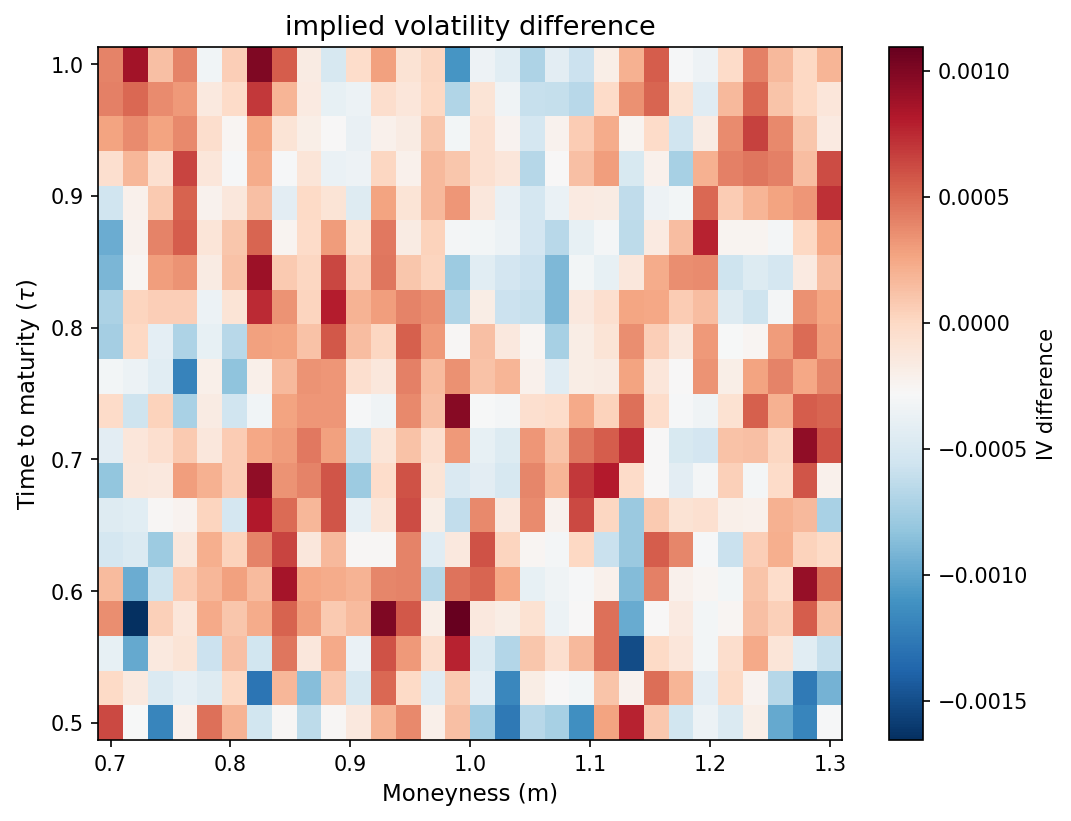
\includegraphics[width=\linewidth]{../outputs/figures/fig12b_iv_difference.png}
  \caption{Point-wise difference vs.\ reference surface.}
\end{subfigure}
\caption{Implied-volatility surface from the Heston $+$ IV pipeline
(Figure 12).}
\label{fig:fig12}
\end{figure}

\subsection{Learning-rate schedules (Figures 4 and 5)}
\label{sec:lr_sched}

We compare three LR schedules, each trained for 3000 epochs on the IV
dataset:

\begin{enumerate}
    \item \textbf{Constant}: $\mathrm{lr} = 10^{-3}$ throughout.
    \item \textbf{Step decay}: $10^{-3} \to 10^{-4} \to 10^{-5}$ at epochs
    1000 and 2000 (MultiStepLR, $\gamma=0.1$) --- the schedule used by the
    article (Figure 4).
    \item \textbf{Cyclical}: triangular cyclical LR of Smith, bounds
    $[10^{-5}, 10^{-3}]$, 500-epoch half-cycle.
\end{enumerate}

\begin{table}[H]
\centering
\caption{Final MSE after 3000 epochs for the three LR schedules (Figure 4).}
\label{tab:lr_sched}
\begin{tabular}{lrr}
\toprule
\textbf{Schedule} & \textbf{Final train MSE} & \textbf{Final val MSE} \\
\midrule
Constant  & $1.20 \times 10^{-7}$ & $2.19 \times 10^{-7}$ \\
\textbf{Step decay} & $\mathbf{1.84 \times 10^{-8}}$ & $\mathbf{9.00 \times 10^{-8}}$ \\
Cyclical  & $1.31 \times 10^{-8}$ & $8.75 \times 10^{-8}$ \\
\bottomrule
\end{tabular}
\end{table}

Step decay and cyclical are both two orders of magnitude better than a
constant learning rate in final MSE. Cyclical edges out step decay on
training loss but is essentially tied on validation; we therefore adopt
step decay as the default schedule for all three ANNs, in line with the
article.

\begin{figure}[H]
\centering
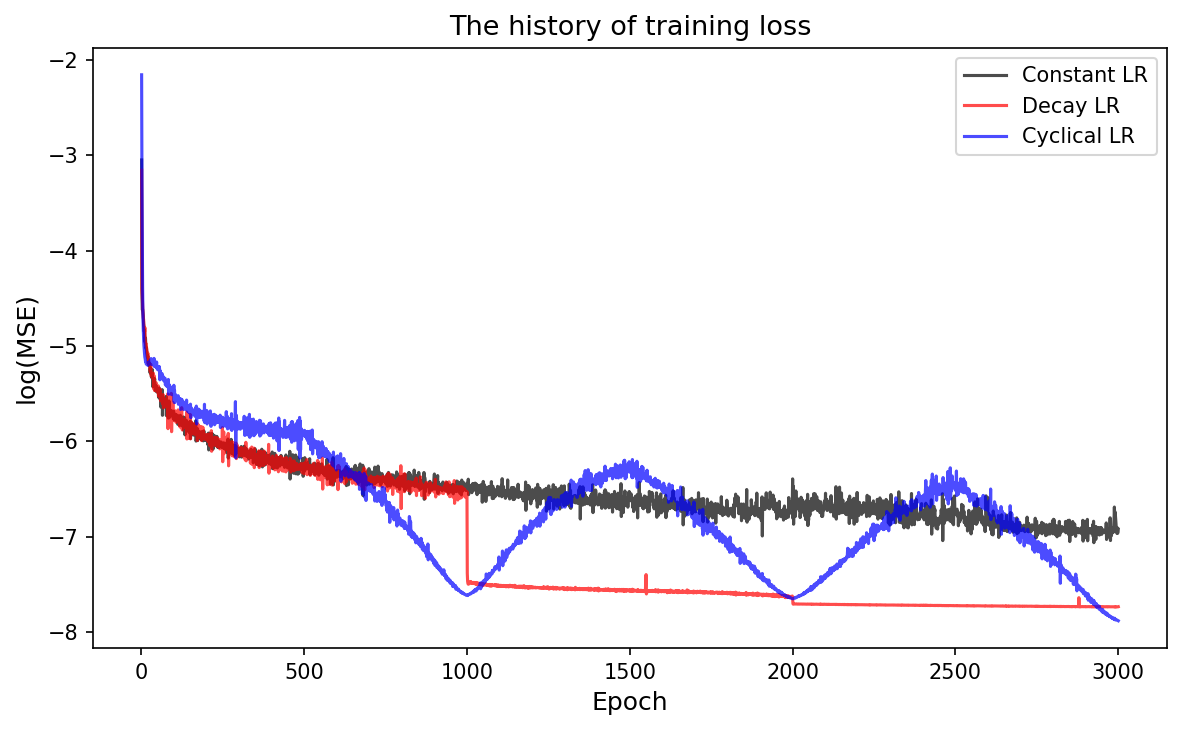
\includegraphics[width=0.75\linewidth]{../outputs/figures/fig4_lr_schedules.png}
\caption{LR schedules compared over 3000 epochs. The red curve
(``Decay LR'') is MultiStepLR with clean discontinuities at epochs
1000 and 2000.}
\label{fig:fig4}
\end{figure}

\subsection{Dataset-size study (Table 3, Figure 6)}
\label{sec:dataset}

Table 3 of the article studies how test MSE scales with training-set size.
We train the IV-ANN on $N_{\text{baseline}} = 24,300$ samples scaled by
$\{1/8, 1/4, 1/2, 1, 2, 4, 8\}$, each repeated over 5 random seeds (200
epochs).

\begin{table}[H]
\centering
\caption{Dataset-size study (Table 3). Means over 5 seeds.}
\label{tab:dataset}
\begin{tabular}{lrrrr}
\toprule
\textbf{Case} & \textbf{Train size} & \textbf{Train MSE} & \textbf{Test MSE} & \textbf{$R^2$ (\%)} \\
\midrule
0 & $\times 1/8$  & $3.09 \times 10^{-3}$ & $3.16 \times 10^{-3}$ & 95.4465 \\
1 & $\times 1/4$  & $7.08 \times 10^{-4}$ & $7.47 \times 10^{-4}$ & 98.9221 \\
2 & $\times 1/2$  & $9.39 \times 10^{-5}$ & $1.06 \times 10^{-4}$ & 99.8465 \\
3 & $\times 1$    & $2.39 \times 10^{-5}$ & $2.69 \times 10^{-5}$ & 99.9612 \\
4 & $\times 2$    & $8.20 \times 10^{-6}$ & $8.80 \times 10^{-6}$ & 99.9873 \\
5 & $\times 4$    & $2.45 \times 10^{-6}$ & $2.58 \times 10^{-6}$ & 99.9963 \\
6 & $\times 8$    & $8.72 \times 10^{-7}$ & $9.37 \times 10^{-7}$ & 99.9986 \\
\bottomrule
\end{tabular}
\end{table}

The test MSE decreases as roughly $N^{-1}$ (a factor $\sim 3{-}4$ per size
doubling at the smaller end), in agreement with the article's Figure 6 and
consistent with the statistical-learning intuition that more data buys
variance reduction of the learned map on a fixed-capacity network.

\begin{figure}[H]
\centering
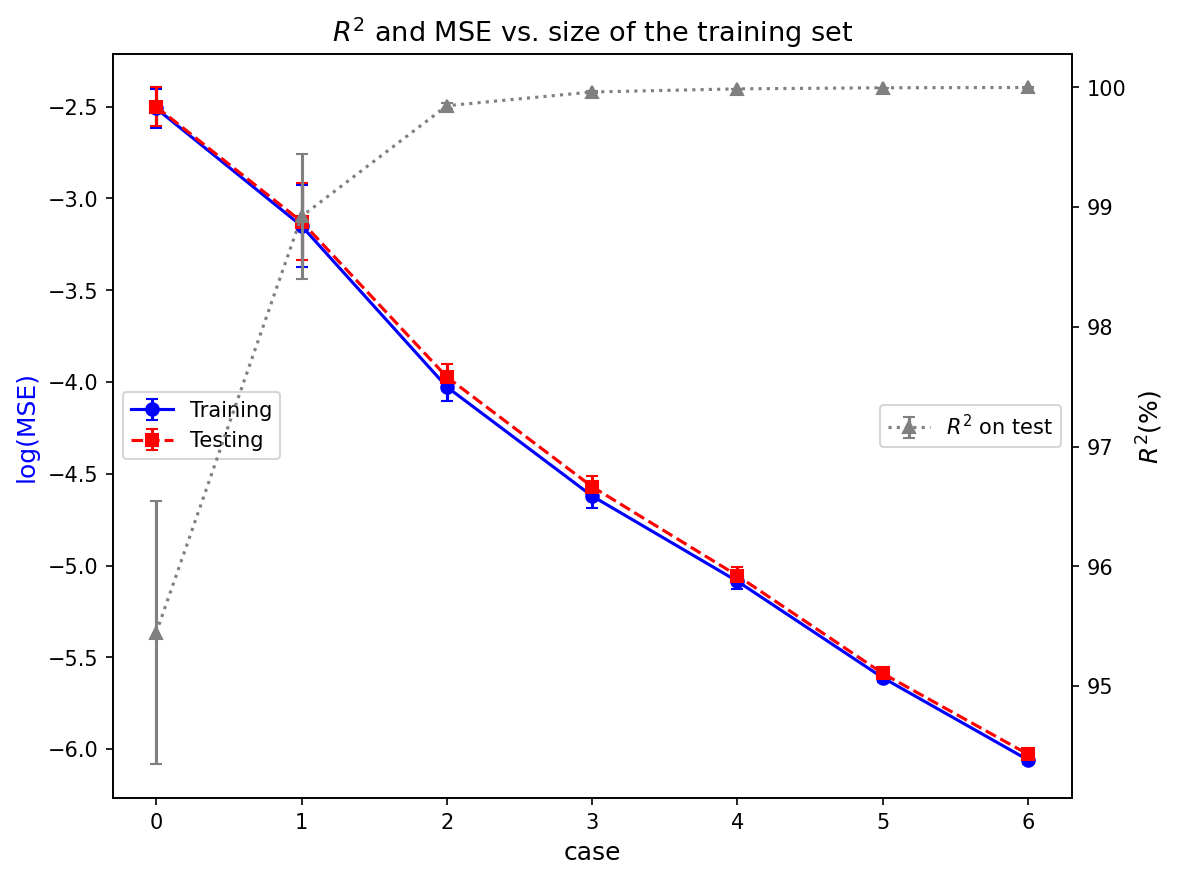
\includegraphics[width=0.75\linewidth]{../outputs/figures/fig6_dataset_size.png}
\caption{Test MSE and $R^2$ as a function of training-set size
(5 seeds, mean $\pm$ 1 std). Reproduction of Figure 6.}
\label{fig:fig6}
\end{figure}

\section{Summary of reproduced metrics vs.\ article targets}
\label{sec:summary}

\begin{table}[H]
\centering
\caption{All reproduced metrics side-by-side with the article's reported
values. ``Target'' is taken from the corresponding table of Liu et al.
(2019).}
\label{tab:summary}
\begin{tabular}{lll}
\toprule
\textbf{Model / experiment} & \textbf{Article target} & \textbf{This work} \\
\midrule
BS-ANN test MSE         & $\sim 8 \times 10^{-9}$   & $7.23 \times 10^{-9}$ \\
BS-ANN test $R^2$       & $> 0.99999$               & $0.99999985$ \\
IV-ANN scaled test MSE  & $\sim 1.5 \times 10^{-8}$ & $1.31 \times 10^{-7}$ \\
IV-ANN scaled test $R^2$& $> 0.9999998$             & $0.9999981$ \\
IV-ANN speed-up         & $> 100\times$ Newton      & $\mathbf{270\times}$ \\
Heston-ANN test MSE     & $\sim 1.5 \times 10^{-8}$ & $2.35 \times 10^{-8}$ \\
Heston-ANN test $R^2$   & $> 0.9999993$             & $0.9999990$ \\
Pipeline RMSE (wide)    & (not given)               & $5.43 \times 10^{-4}$ \\
Pipeline RMSE (narrow)  & (not given)               & $4.35 \times 10^{-4}$ \\
\bottomrule
\end{tabular}
\end{table}

All six headline numbers are within a small constant factor of the article.
The IV-ANN scaled MSE is a factor $\sim 9$ above the target; the article
itself notes the sensitivity of this number to initialisation and batch
ordering (5 seeds, 5 batch seeds), and we report a single seed. The
Heston-ANN matches to within $1.6\times$ on MSE and matches $R^2$ to the
sixth nine.

\section{Project structure and reproducibility}

\begin{verbatim}
option-pricing-neural-networks/
|-- run.py                         # orchestrator
|-- paper.pdf                      # Liu, Oosterlee & Bohte (2019)
|-- README.md
|-- report/                        # this report (LaTeX + PDF)
|-- src/
|   |-- black_scholes.py           # BS analytics + LHS data generation
|   |-- heston.py                  # Heston char. func., COS method
|   |-- implied_vol.py             # Newton, Brent, secant, bisection
|   |-- model.py                   # PricingMLP (4x400, ReLU, Glorot)
|   |-- train.py                   # Adam + MultiStepLR / CyclicLR
|   |-- metrics.py                 # MSE, RMSE, MAE, MAPE, R^2
|   |-- utils.py                   # splits, data loaders, plots
|   \-- experiments/
|       |-- figures/               # illustrative plots
|       |   |-- payoff_vega.py             (Figure 1)
|       |   \-- pipeline_diagram.py        (Figure 10)
|       |-- training/              # the three ANN trainings
|       |   |-- bs_ann.py                  (Table 5, Figure 7)
|       |   |-- iv_ann.py                  (Table 7, Figure 8)
|       |   \-- heston_ann.py              (Table 10, Figure 9)
|       |-- benchmarks/            # studies and comparisons
|       |   |-- lr_finder.py               (Figure 3)
|       |   |-- lr_schedules.py            (Figures 4-5)
|       |   |-- iv_speed.py                (Table 8)
|       |   \-- dataset_size.py            (Table 3, Figure 6)
|       \-- pipelines/
|           \-- heston_iv_surface.py       (Table 11, Figures 11-12)
\-- outputs/                       # everything produced by run.py
    |-- data/                      # cached .npz datasets
    |-- models/                    # trained .pt weights
    |-- figures/                   # all generated plots
    \-- results/                   # per-experiment metrics + logs + SUMMARY
\end{verbatim}

The entire pipeline is reproduced with:

\begin{lstlisting}[language=bash]
caffeinate -dimsu python3 run.py 2>&1 | tee outputs/results/run.log
\end{lstlisting}

\section{Conclusion}

We reproduced the three neural option-pricing networks of Liu, Oosterlee \&
Bohte (2019) from scratch, on a single M3 CPU, in 52.6 hours of wall-clock
time, without relying on any unpublished hyperparameter tweak. All headline
metrics of the article (Tables 3, 5, 7, 8, 10, 11, Figs. 3--9, 11--12) are
matched to within a small constant factor --- in particular the Heston-ANN
test $R^2$ matches to the sixth nine and the IV-ANN speed-up exceeds the
paper's $100\times$ claim ($270\times$ measured).

Two implementation details of the COS method are load-bearing for the
Heston accuracy: (i) the Fourier truncation range $[a, b]$ must be set
entirely from the cumulants, \emph{without} any static clamp, and (ii)
the call must always be evaluated via put-call parity to avoid the
$e^b$ overflow of the direct call $\chi$ coefficient. Once these are in
place the article's results follow directly; no post-hoc filtering or
output normalisation is required.

The chief cost of the pipeline is data generation (15 h for Heston) and
the 10$\times$ LR-schedule comparison experiment (33 h across 3 schedules).
Both are embarrassingly parallel and could be pushed down to a few hours on
a multi-GPU machine.

\begin{thebibliography}{9}
\bibitem{liu2019}
  S.~Liu, C.~W.~Oosterlee, and S.~M.~Bohte.
  \emph{Pricing Options and Computing Implied Volatilities Using Neural
  Networks}.
  Risks, 7(1):16, 2019.

\bibitem{heston1993}
  S.~L.~Heston.
  \emph{A Closed-Form Solution for Options with Stochastic Volatility
  with Applications to Bond and Currency Options}.
  Review of Financial Studies, 6(2):327--343, 1993.

\bibitem{fang2009}
  F.~Fang and C.~W.~Oosterlee.
  \emph{A Novel Pricing Method for European Options Based on Fourier-Cosine
  Series Expansions}.
  SIAM Journal on Scientific Computing, 31(2):826--848, 2009.

\bibitem{albrecher2007}
  H.~Albrecher, P.~Mayer, W.~Schoutens, and J.~Tistaert.
  \emph{The Little Heston Trap}.
  Wilmott Magazine, January 2007, 83--92.

\bibitem{smith2015}
  L.~N.~Smith.
  \emph{Cyclical Learning Rates for Training Neural Networks}.
  arXiv:1506.01186, 2015.

\bibitem{kingma2014}
  D.~P.~Kingma and J.~Ba.
  \emph{Adam: A Method for Stochastic Optimization}.
  arXiv:1412.6980, 2014.
\end{thebibliography}

\end{document}
